\section{Varianz}
\label{section-varianz}
\kopfrechts{Varianz}
\index{Varianz}
Die Qualitätskontrolle bei der Herstellung von Widerständen versucht
ein Mass dafür zu entwickeln, wie genau die produzierten Widerstände
den beabsichtigen Widerstandswert einhalten. 
Dazu werden der Produktion einige Widerstände entnommen und ihr Wert
nachgemessen.
Den Erwartungswert des Widerstandswertes kann man mit
Hilfe des Mittelwertes abschätzen, er sollte ungefähr mit dem Sollwert
übereinstimmen.
Wie aber kann man die ``Streuung'' der Widerstandswerte
bewerten?

Als weiteres Beispiel betrachten wir die Zufallsvariable $X$
``Messung einer Spannung''.
Nicht jede Messung ergibt den gleichen Wert,
das Signal ist von einem Rauschen überlagert.
Der Mittelwert der
Messwert entspricht gemäss dem vorangegangenen Abschnitt dem Erwartungswert
$E(X)$.
Wie aber soll das Ausmass des Rauschens gemessen werden?
Ein praktischer Ansatz besteht darin, nach der Energie zu fragen, die
in dem Rauschsignal steckt.
Die Leistung einer Wechselspannung $U(t)$
an einem Widerstand $R$ ist ja
$\frac{U(t)^2}R$, d.~h.~die mittlere Leistung während des Intervalls $[t_0,t_1]$ 
ist
\[
\frac1{t_1-t_0}\int_{t_0}^{t_1}\frac{U(t)^2}R\,dt.
\]
Stellen wir uns vor, dass die Spannungsmessung $X$ in regelmässigen, kurzen
Zeitintervallen wiederholt wird, dann ist die mittlere Leistung
des Differenzsignals $X-E(X)$ also proportional zur Summe der Quadrate
der Werte $(X-E(X))^2$, oder
\[
E((X-E(X))^2).
\]

\subsection{Definition}
\index{Varianz!Definition}
Die Einführungsbespiele motivieren folgende Definition:
\begin{definition}
Sei $X\colon\Omega\to\mathbb{R}$ eine Zufallsvariable, dann
heisst die durch $\operatorname{var}(X)^2=E((X-E(X))^2)$ definierte Grösse $\operatorname{var}(X)$ die
{\em Varianz} von $X$.
Es ist insbesondere
\[
\operatorname{var}(X)=E((X-E(X))^2)=E(X^2)-E(X)^2
\]
\end{definition}
Die letzte Gleichung kann man leicht nachrechnen:
\begin{align*}
\operatorname{var}(X)&=E((X-E(X))^2)\\
&=E(X^2-2XE(X)+E(X)^2)\\
&=E(X^2)-2E(X)E(X)+E(X)^2\\
&=E(X^2)-E(X)^2.
\end{align*}
%%
\begin{figure}
\begin{center}
%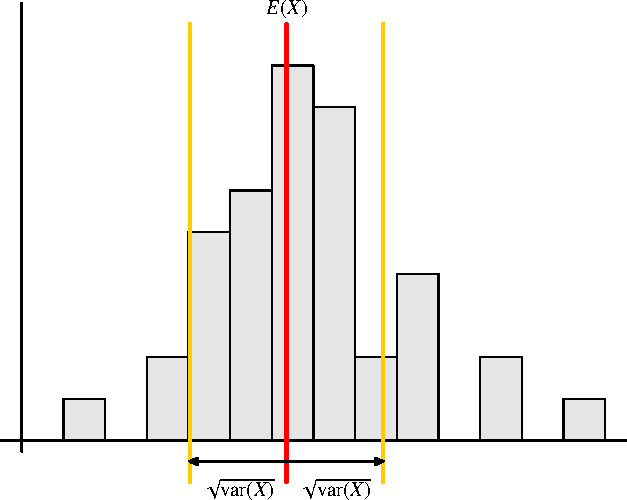
\includegraphics[width=\hsize]{images/erwartung-1}
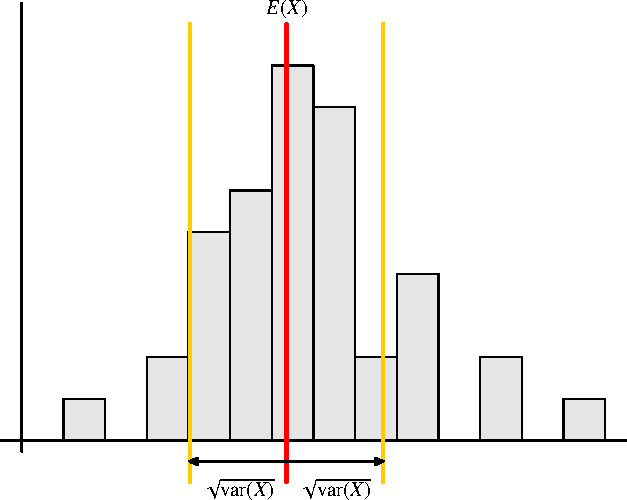
\includegraphics{images/erwartung-1}
\end{center}
\caption{Visualisierung von Erwartungswert und Varianz in einem Histogramm
\label{histogram}}
\end{figure}%

Man beachte, dass $\operatorname{var}(X)$ die Masseinheit des Quadrates
von $X$ hat.
Wenn also $X$ als Masseinheit eine Länge hat,
dann hat $\operatorname{var}(X)$ die Masseinheit einer Fläche.
Insbesondere kann man $\operatorname{var}(X)$ nicht in der gleichen
Zeichnung visualisieren wie $E(X)$.
Aber die Grösse $\sqrt{\operatorname{var}(X)}$ hat die gleiche Masseinheit, sie
drückt die ``Streubreite'' der Werte von $X$ aus,
wie in Abbildung~\ref{histogram} veranschaulicht.

Die Definition der Varianz ``passt'' in natürlicher Weise zum Erwartungswert,
wie der folgende Satz zeigt:
\begin{satz}\label{erwartungswert-charakterisierung}
Der Erwartungswert $E(X)$ einer reellen Zufallsvariable $X$ ist diejenige
reelle Zahl $\mu$, für die $E((X-\mu)^2)$ minimal wird.
\end{satz}
\begin{proof}[Beweis]
Aus den Rechenregeln finden wir
\begin{align*}
E((X-\mu)^2)
&=
E(X^2-2\mu X+\mu^2)
\\
&=
E(X^2)-2\mu E(X) +\mu^2E(1)
\\
&=
E(X^2)-2\mu E(X) +\mu^2
\end{align*}
Dies ist eine quadratische Funktion, die ihren Scheitelpunkt bei $\mu$ hat.
Man kann dies auch durch Nullsetzen der Ableitung nach $\mu$ finden:
\[
\frac{d}{d\mu}\left(E(X^2)-2\mu E(X) +\mu^2\right)=-2 E(X)+2\mu=0,
\]
Auflösen nach $\mu$ ergibt $\mu=E(X)$.
\end{proof}
Wir wenden die Definition der Varianz auf das Beispiel der Widerstandsmessung
an,
Wir haben bereits im Abschnitt \ref{erwartungswertvonmesswerten}
den Erwartungswert $E(R)=0.99015$ der Widerstandsmesswerte ermittelt, darauf aufbauend
können wir jetzt auch die Varianz berechnen.
Man findet zum Beispiel die Widerstandswerte gemäss
Tabelle~\ref{varianzberechnung}.
\begin{table}
\begin{center}
\begin{tabular}{|c|r|r|r|}
\hline
Nummer&Messwert&Abweichung&$\text{Abweichung}^2$\\
\hline
1&0.990&-0.00015&0.0000000225\\
2&0.989&-0.00115&0.0000013225\\
3&0.991&0.00085&0.0000007225\\
4&0.991&0.00085&0.0000007225\\
5&0.991&0.00085&0.0000007225\\
6&0.989&-0.00115&0.0000013225\\
7&0.990&0.00015&0.0000000225\\
8&0.989&-0.00115&0.0000013225\\
9&0.992&0.00185&0.0000034225\\
10&0.992&0.00185&0.0000034225\\
11&0.990&-0.00015&0.0000000225\\
12&0.989&-0.00115&0.0000013225\\
13&0.990&-0.00015&0.0000000225\\
14&0.991&0.00085&0.0000007225\\
15&0.989&-0.00115&0.0000013225\\
16&0.990&-0.00015&0.0000000225\\
17&0.989&-0.00115&0.0000013225\\
18&0.990&-0.00015&0.0000000225\\
19&0.990&-0.00015&0.0000000225\\
20&0.991&0.00085&0.0000007225\\
\hline
&$\mu=1.000$&$\sigma=0.000963$&
$\sigma^2=0.0000009275$\\
\hline
\end{tabular}
\end{center}
\caption{Einzelmessungen an Widerständen und Berechnung der Varianz
\label{varianzberechnung}}
\end{table}

\subsubsection{Beispiel: Wurf einer fairen Münze}
Beim Wurf einer fairen Münze werde der Gewinn $1$ ausbezahlt bei
``Kopf'', bei ``Zahl'' wird hingegen $0$ ausbezahlt.
Es ist klar, dass die erwartete Auszahlung $E(X)=\frac12$ ist.
Daraus lässt sich jetzt auch die Varianz berechnen:
\begin{align*}
\operatorname{var}(X)
&=
E((X-E(X))^2)=E\biggl(\biggl(X-\frac12\biggr)^2\biggr)
=\frac12\cdot \biggl(1-\frac12\biggr)^2+\frac12\biggl(0-\frac12\biggr)^2\\
&=\frac12\cdot\frac14+\frac12\cdot\frac14=\frac14.
\end{align*}

\subsubsection{Varianz eines Würfels}
Ist $X$ die Augenzahl eines fairen Würfels, dann ist der
Erwartungswert  $E(X)=\frac{7}2$ bereits bekannt.
Für die Berechnung der Varianz muss zusätzlich $E(X^2)$ ermittelt
werden.
Dazu werden die Werte quadriert, die Wahrscheinlichkeiten bleiben gleich:
\begin{align*}
E(X^2)
&=
\frac16 \cdot 1^2
+
\frac16 \cdot 2^2
+
\frac16 \cdot 3^2
+
\frac16 \cdot 4^2
+
\frac16 \cdot 5^2
+
\frac16 \cdot 6^2
\\
&=
\frac16\cdot( 1+4+9+16+25+36)
=
\frac{91}{6}
\\
\operatorname{var}(X)
&=
E(X)^2-E(X)^2
=
\frac{91}{6}-\biggl(\frac{7}{2}\biggr)^2
=
\frac{91}{6}-\frac{49}{4}
=
\frac{182-147}{12}=\frac{35}{12}.
\end{align*}

\subsection{Empirische Berechnung}
\index{Varianz!angenäherte Berechnung}
Wir betrachten das praktische Beispiel der Bestimmung der Varianz
einer Messreihe.
Gegeben sind also die Messwerte $(x_i)_{1\le i\le n}$
Auf den ersten Blick sieht es so aus, als wäre für die Berechnung der Varianz
sehr viel Speicherplatz erforderlich.
Zwar ist für die Berechnung des
Erwartungswertes von $\mu=E(X)=\frac1n\sum_{i=1}^n x_i$ kein besonderer Aufwand
notwendig, da die Summe laufend gebildet werden kann.
Zur Berechnung der
Varianz muss aber erst $\mu$ bestimmt werden, bevor man die Differenzen $(x_i-\mu)$
bilden kann.
Trotzdem lässt sich die Berechnung vereinfachen:
\begin{align*}
E((X-\mu)^2)&=\frac1n\sum_{i=1}^n(x_i-\mu)^2\\
&=\frac1n\sum_{i=1}^n(x_i^2-2\mu x_i+\mu^2)\\
&=\frac1n\sum_{i=1}^nx_i^2-2\mu\frac1n\sum_{i=1}^n x_i+\mu^2\\
&=\frac1n\sum_{i=1}^nx_i^2-\biggl(\frac1n\sum_{i=1}^nx_i\biggr)^2.
\end{align*}
\subsubsection{Beobachtungen}
\begin{enumerate}
\item
Es genügt also, $x_i$ und $x_i^2$ zu summieren, wozu nur zwei Speicherplätze
benötigt werden.
Aus den beiden Summen kann die Varianz bereits berechnet werden.
Es ist nicht nötig, die einzelnen Messwerte $x_i$ zu speichern.
\item
Die Berechnung der Varianz kann also ganz einfach mit einer Tabelle
erfolgen:
\begin{center}
%\begin{tabular}{|>{$}c<{$}|>{$}c<{$}|}
\begin{tabular}{|c|c|c|}
\hline
$i$&$x_i$&$x_i^2$\\
\hline
$1$&$x_1$&$x_1^2$\\
$2$&$x_2$&$x_2^2$\\
$\vdots$&$\vdots$&$\vdots$\\
$n$&$x_n$&$x_n^2$\\
\hline
&$\sum_{i=0}^n x_i$&$\sum_{i=0}^n x_i^2$\\
\hline
\end{tabular}
\end{center}
\item
Grosse Abweichungen können vorkommen, und bekommen wegen des
Quadrates in der Varianz auch grosses Gewicht.
Hat man aber nur
wenige Messwerte, ist es unwahrscheinlich, eine solche grosse
Abweichung, einen ``Ausreisser'', zu sehen.
Daher unterschätzt
diese empirische Formel den tatsächlichen Wert der Varianz immer
dann, wenn $n$ klein ist.
Wir werden später sehen, dass eine
besser Schätzung zu bekommen ist, wenn man noch einen Korrekturfaktor
$\frac{n}{n-1}$ hinzufügt.
\end{enumerate}

\subsection{Weitere Rechenregeln}
\begin{satz}
\label{rechenregeln-varianz}
Seien $X$ und $Y$ unabhängige Zufallsvariable, dann haben
Summe und Produkt folgende Varianz:
\begin{align*}
\operatorname{var}(\lambda X)&=\lambda^2\operatorname{var}(X)\\
\operatorname{var}(X+Y)&=\operatorname{var}(X)+\operatorname{var}(Y)\\
\operatorname{var}(XY)&=\operatorname{var}(X)\operatorname{var}(Y)
+
\operatorname{var}(Y)E(X)^2+\operatorname{var}(X)E(Y)^2.
\end{align*}
\end{satz}
\begin{proof}[Beweis]Durch einfaches Nachrechnen unter Ausnützen der
Rechenregeln für den Erwartungswert und der
Unabhängigkeit von $X$ und $Y$, d.~h.~$E(XY)=E(X)E(Y)$:
\begin{align*}
\operatorname{var}(X+Y)
&=E((X+Y)^2)-E(X+Y)^2\\
&=E(X^2+2XY+Y^2)-(E(X)+E(Y))^2\\
&=E(X^2)+2E(XY)+E(Y^2)-E(X)^2-2E(X)E(Y)-E(Y)^2\\
&=E(X^2)-E(X)^2+E(Y^2)-E(Y)^2\\
&=\operatorname{var}(X)+\operatorname{var}(Y).
\end{align*}
Durch Ziehen der Wurzel folgt die Behauptung aus der letzten Gleichung.
Für das Produkt gilt
\begin{align*}
\operatorname{var}(XY)
&=E(X^2Y^2)-E(XY)^2\\
&=E(X^2)E(Y^2)-E(X)^2E(Y)^2\\
&=(\operatorname{var}(X)+E(X)^2)(\operatorname{var}(Y)+E(Y)^2)
-E(X)^2E(Y)^2\\
&=\operatorname{var}(X)\operatorname{var}(Y)+E(X)^2\operatorname{var}(Y)
+\operatorname{var}(X)E(Y)^2
\end{align*}
und daraus die Behauptung.
\end{proof}

\subsubsection{Beobachtungen}

\begin{enumerate}
\item
Die Varianz funktioniert ähnlich wie das Quadrieren für gewöhnliche Zahlen.
Schreibt man $E(XY)-E(X)E(Y)=\operatorname{cov}(X,Y)$, lautete die
binomische Formel wird für die Varianz:
\begin{equation}
\operatorname{var}(X+Y)=\operatorname{var}(X)
+2\operatorname{cov}(X,Y)
+\operatorname{var}(Y).
\label{var-summe-abhaengig}
\end{equation}
Die Kovarianz $\operatorname{cov}(X,Y)$ spielt also die Rolle des gemischten
Terms in der ``gewöhnliche'' binomischen Formel.
\item
Sind $X$ und $Y$ unabhängig, gilt daher die Formel
\begin{align*}
\operatorname{var}(X+Y)
&=
\operatorname{var}(X)
+
\operatorname{var}(Y),
\\
\sqrt{\operatorname{var}(X+Y)}
&=
\sqrt{
\sqrt{\operatorname{var}(X)}^2
+
\sqrt{\operatorname{var}(Y)}^2
}.
\end{align*}
Die Grössen $\sqrt{\operatorname{var}(X)}$ und $\sqrt{\operatorname{var}(Y)}$
werden daher wie die Katheten eines rechtwinkligen Dreiecks addiert,
man spricht von {\it pythagoräischer} Addition.
\end{enumerate}

\subsubsection{Anwendung: Wurf von \texorpdfstring{$n$}{n} Münzen}
Sei $X$ die Anzahl ``Kopf'' beim Wurf von $n$ Münzen.
Natürlich wird
$X$ nur Werte zwischen $0$ und $n$ annehmen.
Zur Berechnung von $E(X)$ und $\operatorname{var}(X)$ wollen wir
die Rechenregeln verwenden.
Dabei verwenden wir neue Zufallsvariablen
$X_i$ wie folgt:
\begin{center}
\begin{tabular}{clcc}
$X_1$&Anzahl Kopf im ersten Wurf&$E(X_1)=\frac12$&$\operatorname{var}(X_1)=\frac14$\\
$X_2$&Anzahl Kopf im zweiten Wurf&$E(X_2)=\frac12$&$\operatorname{var}(X_2)=\frac14$\\
&$\dots$&&\\
$X_n$&Anzahl Kopf im $n$-ten Wurf&$E(X_n)=\frac12$&$\operatorname{var}(X_n)=\frac14$.
\end{tabular}
\end{center}
Damit kann man Erwartungswert und Varianz von $X=X_1+X_2+\dots+X_n$ berechnen:
\begin{align*}
E(X)&=
E(X_1)+
E(X_2)+\dots+
E(X_n)
=
\frac{1}2+
\frac{1}2+\dots+
\frac{1}2=\frac{n}2,
\\
\operatorname{var}(X)
&=
\operatorname{var}(X_1)
+
\operatorname{var}(X_2)
+\dots+
\operatorname{var}(X_n)
=\frac14+\frac14+\dots+\frac14=\frac{n}4.
\end{align*}

